\begin{figure}
    \centering
    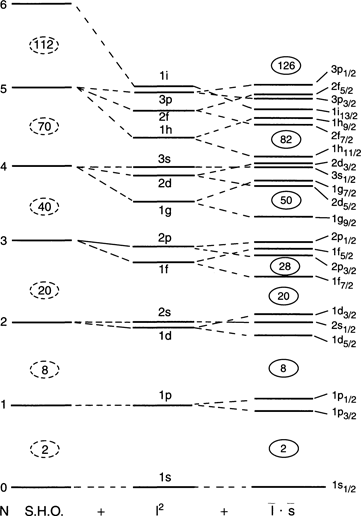
\includegraphics[scale=2]{Introduction_Figs/ShellBreakdownCasten.png}
    \caption{The evolution of the shel model and the creation of the closed shells of a spherical nucleus. On the left is the spherical harmonic oscillator. By adding in an angular momentum term, some of the degenerate levels separate. By further adding a spin-coupling term, the levels separate with energy spacings that create the closed shells and the magic numbers. Taken from \citep{casten90:_structure}.}
    \label{fig:shellmodel}
\end{figure}